%!Mode:: "TeX:UTF-8"
%!TEX encoding = UTF-8 Unicode
%lan
%arara: xelatex
\documentclass{ctexart}
\newif\ifpreface
%\prefacetrue
\input{../../../global/all}
\begin{document}
\large
\setlength{\baselineskip}{1.2em}
\ifpreface
\input{../../../global/preface}
\newgeometry{left=2cm,right=2cm,top=2cm,bottom=2cm}
\else
\newgeometry{left=2cm,right=2cm,top=2cm,bottom=2cm}
\maketitle
\fi
%from_here_to_type
\begin{problem}\label{pro:1}
  Use the Taylor series to show that the approximation
  \[
    \frac{\partial}{\partial x}
    \left(
      a\frac{\partial u}{\partial x}
    \right)(x_i,y_j)
    \approx
    \frac{
      a_{i+\frac12,j}(u_{i+1,j}-u_{i,j})
      -
      a_{i-\frac12,j}(u_{i,j}-u_{i-1,j})
    }{
      h_x^2
    }
  \]
  is second-order accurate, provided that
  \[
    a\frac{\partial u}{\partial x}\in C^3,
    \qquad
    a\frac{\partial^3 u}{\partial x^3}\in C^1.
  \]

  That is, show that the absolute value of the difference between the
  right-hand side and left-hand side is bounded by
  \[
    \frac{h_x^2}{24}
    \left[
      \max_{x\in[x_{i-1},x_{i+1}]}
      \left|
      \frac{\partial^3}{\partial x^3}
      \left(
        a\frac{\partial u}{\partial x}
      \right)
      \right|
      +
      \max_{x\in[x_{i-1},x_{i+1}]}
      \left|
      \frac{\partial}{\partial x}
      \left(
        a\frac{\partial^3 u}{\partial x^3}
      \right)
      \right|
    \right].
  \]
\end{problem}
\begin{lemma}[Midpoint Taylor expansion]
  Let \(u\) be sufficiently smooth on \([x_i,x_{i+1}]\), and let
  \[
    x_{i+\frac12}=x_i + \frac{h}{2},x_{i + 1}= x_i + h.
  \]
  Then
  \[
    \frac{u_{i+1,j}-u_{i,j}}{h}
    =
    u_x(x_{i+\frac12},y_j)
    +
    \frac{h^2}{24}
    u_{xxx}(x_{i+\frac12},y_j)
    +
    O(h^4).
  \]
  Similarly,
  \[
    \frac{u_{i,j}-u_{i-1,j}}{h}
    =
    u_x(x_{i-\frac12},y_j)
    +
    \frac{h^2}{24}
    u_{xxx}(x_{i-\frac12},y_j)
    +
    O(h^4).
  \]
\end{lemma}

\begin{proof}
  We prove the first formula. Let
  \[
    m=x_{i+\frac12}.
  \]
  Then
  \[
    x_{i+1}=m+\frac{h}{2},
    \qquad
    x_i=m-\frac{h}{2}.
  \]
  Taylor expansion about \(m\) gives
  \[
    u(x_{i+1},y_j)
    =
    u(m,y_j)
    +
    \frac{h}{2}u_x(m,y_j)
    +
    \frac{h^2}{8}u_{xx}(m,y_j)
    +
    \frac{h^3}{48}u_{xxx}(m,y_j)
    +
    O(h^4),
  \]
  and
  \[
    u(x_i,y_j)
    =
    u(m,y_j)
    -
    \frac{h}{2}u_x(m,y_j)
    +
    \frac{h^2}{8}u_{xx}(m,y_j)
    -
    \frac{h^3}{48}u_{xxx}(m,y_j)
    +
    O(h^4).
  \]
  Subtracting the two expansions yields
  \[
    u_{i+1,j}-u_{i,j}
    =
    hu_x(m,y_j)
    +
    \frac{h^3}{24}u_{xxx}(m,y_j)
    +
    O(h^5).
  \]
  Dividing by \(h\), we obtain
  \[
    \frac{u_{i+1,j}-u_{i,j}}{h}
    =
    u_x(x_{i+\frac12},y_j)
    +
    \frac{h^2}{24}u_{xxx}(x_{i+\frac12},y_j)
    +
    O(h^4).
  \]
  The second formula is proved in the same way.
\end{proof}

\begin{solution}[Proof of the approximation]
  Fix \(y=y_j\), and write
  \[
    h=h_x.
  \]
  Define
  \[
    F(x)=a(x,y_j)u_x(x,y_j),
    \qquad
    G(x)=a(x,y_j)u_{xxx}(x,y_j).
  \]
  Then
  \[
    F'(x_i)
    =
    \frac{\partial}{\partial x}
    \left(
      a\frac{\partial u}{\partial x}
    \right)(x_i,y_j).
  \]

  By the midpoint Taylor expansion lemma,
  \[
    \frac{u_{i+1,j}-u_{i,j}}{h}
    =
    u_x(x_{i+\frac12},y_j)
    +
    \frac{h^2}{24}u_{xxx}(x_{i+\frac12},y_j)
    +
    O(h^4),
  \]
  and
  \[
    \frac{u_{i,j}-u_{i-1,j}}{h}
    =
    u_x(x_{i-\frac12},y_j)
    +
    \frac{h^2}{24}u_{xxx}(x_{i-\frac12},y_j)
    +
    O(h^4).
  \]

  Multiplying by \(a_{i+\frac12,j}\) and \(a_{i-\frac12,j}\), respectively, gives
  \[
    a_{i+\frac12,j}
    \frac{u_{i+1,j}-u_{i,j}}{h}
    =
    F(x_{i+\frac12})
    +
    \frac{h^2}{24}G(x_{i+\frac12})
    +
    O(h^4),
  \]
  and
  \[
    a_{i-\frac12,j}
    \frac{u_{i,j}-u_{i-1,j}}{h}
    =
    F(x_{i-\frac12})
    +
    \frac{h^2}{24}G(x_{i-\frac12})
    +
    O(h^4).
  \]

  Subtracting and dividing by \(h\), we obtain
  \[
    \begin{aligned}
      &
      \frac{
        a_{i+\frac12,j}(u_{i+1,j}-u_{i,j})
        -
        a_{i-\frac12,j}(u_{i,j}-u_{i-1,j})
      }{h^2}
      \\
      &=
      \frac{
        F(x_{i+\frac12})-F(x_{i-\frac12})
      }{h}
      +
      \frac{h^2}{24}
      \frac{
        G(x_{i+\frac12})-G(x_{i-\frac12})
      }{h}
      +
      O(h^3).
    \end{aligned}
  \]

  Now, by the centered difference formula,
  \[
    \frac{
      F(x_{i+\frac12})-F(x_{i-\frac12})
    }{h}
    =
    F'(x_i)
    +
    \frac{h^2}{24}F'''(\eta)
  \]
  for some
  \[
    \eta\in(x_{i-1},x_{i+1}).
  \]

  Also, by the mean value theorem,
  \[
    \frac{
      G(x_{i+\frac12})-G(x_{i-\frac12})
    }{h}
    =
    G'(\zeta)
  \]
  for some
  \[
    \zeta\in(x_{i-1},x_{i+1}).
  \]

  Therefore,
  \[
    \begin{aligned}
      &
      \frac{
        a_{i+\frac12,j}(u_{i+1,j}-u_{i,j})
        -
        a_{i-\frac12,j}(u_{i,j}-u_{i-1,j})
      }{h^2}
      -
      F'(x_i)
      \\
      &=
      \frac{h^2}{24}F'''(\eta)
      +
      \frac{h^2}{24}G'(\zeta)
      +
      O(h^3).
    \end{aligned}
  \]

  Taking absolute values gives
  \[
    \begin{aligned}
      &
      \left|
      \frac{
        a_{i+\frac12,j}(u_{i+1,j}-u_{i,j})
        -
        a_{i-\frac12,j}(u_{i,j}-u_{i-1,j})
      }{h^2}
      -
      F'(x_i)
      \right|
      \\
      &\le
      \frac{h^2}{24}
      \max_{x\in[x_{i-1},x_{i+1}]}
      |F'''(x)|
      +
      \frac{h^2}{24}
      \max_{x\in[x_{i-1},x_{i+1}]}
      |G'(x)|
      +
      O(h^3).
    \end{aligned}
  \]

  Since
  \[
    F(x)=a(x,y_j)u_x(x,y_j) \in C^3,
    \qquad
    G(x)=a(x,y_j)u_{xxx}(x,y_j) \in C^1,
  \]
  we have
  \[
    F'''(x)
    =
    \frac{\partial^3}{\partial x^3}
    \left(
      a\frac{\partial u}{\partial x}
    \right)(x,y_j),
  \]
  and
  \[
    G'(x)
    =
    \frac{\partial}{\partial x}
    \left(
      a\frac{\partial^3u}{\partial x^3}
    \right)(x,y_j).
  \]

  Thus
  \[
    \begin{aligned}
      &
      \left|
      \frac{
        a_{i+\frac12,j}(u_{i+1,j}-u_{i,j})
        -
        a_{i-\frac12,j}(u_{i,j}-u_{i-1,j})
      }{h_x^2}
      -
      \frac{\partial}{\partial x}
      \left(
        a\frac{\partial u}{\partial x}
      \right)(x_i,y_j)
      \right|
      \\
      &\le
      \frac{h_x^2}{24}
      \left[
        \max_{x\in[x_{i-1},x_{i+1}]}
        \left|
        \frac{\partial^3}{\partial x^3}
        \left(
          a\frac{\partial u}{\partial x}
        \right)
        \right|
        +
        \max_{x\in[x_{i-1},x_{i+1}]}
        \left|
        \frac{\partial}{\partial x}
        \left(
          a\frac{\partial^3u}{\partial x^3}
        \right)
        \right|
      \right]
      +
      O(h_x^3).
    \end{aligned}
  \]

  Hence the approximation is second-order accurate.
\end{solution}
\begin{problem}\label{pro:2}

  Let $u(x,y)$ be the solution of Poisson's equation

  \[
    -\Delta u = f
  \]

  on the unit square with homogeneous Dirichlet boundary conditions

  \[
    u(x,0)=u(x,1)=u(0,y)=u(1,y)=0,
  \]

  and let $\mathbf{u}$ be the vector of values
  $u(x_i,y_j)$ (using natural ordering) on a uniform grid of spacing
  $h$ in each direction.

  Let $\hat{\mathbf{u}}$ be the solution of the linear system

  \[
    -\Delta_h \hat{\mathbf{u}} = \mathbf{f},
  \]

  where $-\Delta_h=A$ is the block tridiagonal matrix

  \[
    A=
    \begin{pmatrix}
      S & T &   &   &   \\
      T & S & T &   &   \\
      & \ddots & \ddots & \ddots & \\
      &   & T & S & T \\
      &   &   & T & S
    \end{pmatrix},
  \]

  with

  \[
    T=-\frac1{h^2}I,
  \]

  and

  \[
    S=
    \begin{pmatrix}
      d & b &   &   &   \\
      b & d & b &   &   \\
      & \ddots & \ddots & \ddots & \\
      &   & b & d & b \\
      &   &   & b & d
    \end{pmatrix},
    \qquad
    d=\frac4{h^2},
    \qquad
    b=-\frac1{h^2}.
  \]

  Here $\mathbf{f}$ is the vector of right-hand-side values
  $f(x_i,y_j)$.

  Use the previous exercise and the estimate for the eigenvalues of $A$
  to show that

  \[
    \sqrt{
      \frac1n
      \sum_{i=1}^{n}
      \left(u_i-\hat{u}_i\right)^2
    }
    \le C h^2,
  \]

  for some constant $C$ independent of $h$.

\end{problem}
\begin{solution}

  Let
  \[
    e=\mathbf u-\hat{\mathbf u}
  \]
  denote the discretization error.

  Since the five-point finite difference approximation of the Laplacian
  is second-order accurate, the exact solution satisfies

  \[
    -\Delta_h \mathbf u
    =
    \mathbf f+\boldsymbol\tau,
  \]

  where \(\boldsymbol\tau\) is the local truncation error vector.
  Moreover, if \(u\in C^4(\Omega)\), then

  \[
    |\tau_i|
    \le
    C_1 h^2,
    \qquad
    i=1,\ldots,n,
  \]

  for some constant \(C_1\) independent of \(h\).
  Consequently,

  \[
    \norm{\boldsymbol\tau}_2
    \le
    \sqrt n\, C_1 h^2,
  \]

  or equivalently,

  \[
    \frac1{\sqrt n}\norm{\boldsymbol\tau}_2
    \le
    C_1 h^2.
  \]

  Since \(A=-\Delta_h\), the sampled exact solution and the numerical
  solution satisfy

  \[
    A\mathbf u
    =
    \mathbf f+\boldsymbol\tau,
    \qquad
    A\hat{\mathbf u}
    =
    \mathbf f .
  \]

  Subtracting the two equations yields

  \[
    Ae
    =
    A(\mathbf u-\hat{\mathbf u})
    =
    \boldsymbol\tau .
  \]

  Since \(A\) is nonsingular,

  \[
    e
    =
    A^{-1}\boldsymbol\tau .
  \]

  Taking the Euclidean norm gives

  \[
    \norm{e}_2
    \le
    \norm{A^{-1}}_2
    \,\norm{\boldsymbol\tau}_2 .
  \]

  Therefore, it remains to estimate \(\norm{A^{-1}}_2\).

  For the two-dimensional discrete Laplacian, the eigenvalues are

  \[
    \lambda_{pq}
    =
    \frac4{h^2}
    \left(
      \sin^2
      \frac{p\pi}{2(m+1)}
      +
      \sin^2
      \frac{q\pi}{2(m+1)}
    \right),
    \qquad
    1\le p,q\le m .
  \]

  Hence the smallest eigenvalue is

  \[
    \lambda_{\min}(A)
    =
    \frac8{h^2}
    \sin^2
    \frac{\pi}{2(m+1)} .
  \]

  Since

  \[
    h=\frac1{m+1},
  \]

  we obtain

  \[
    \lambda_{\min}(A)
    =
    \frac8{h^2}
    \sin^2
    \left(\frac{\pi h}{2}\right).
  \]

  Using the estimate

  \[
    \sin x \ge \frac{2}{\pi}x,
    \qquad
    0\le x\le \frac{\pi}{2},
  \]

  with \(x=\pi h/2\), we find

  \[
    \lambda_{\min}(A)
    \ge
    \frac8{h^2}
    \left(\frac{2}{\pi}\frac{\pi h}{2}\right)^2
    =
    8 .
  \]

  Therefore

  \[
    \norm{A^{-1}}_2
    =
    \frac1{\lambda_{\min}(A)}
    \le
    \frac18 ,
  \]

  which is bounded independently of \(h\).

  Combining this estimate with the truncation-error bound gives

  \[
    \norm{e}_2
    \le
    C\,\norm{\boldsymbol\tau}_2 .
  \]

  Dividing by \(\sqrt n\), we obtain

  \[
    \frac1{\sqrt n}\norm{e}_2
    \le
    C
    \frac1{\sqrt n}
    \norm{\boldsymbol\tau}_2
    \le
    C h^2 .
  \]

  Finally,

  \[
    \frac1{\sqrt n}\norm{e}_2
    =
    \sqrt{
      \frac1n
      \sum_{i=1}^n
      (u_i-\hat u_i)^2
    },
  \]

  and therefore

  \[
    \boxed{
      \sqrt{
        \frac1n
        \sum_{i=1}^n
        (u_i-\hat u_i)^2
      }
      \le
      C h^2 .
    }
  \]

  Thus the discrete solution converges to the exact solution with
  second-order accuracy in the root-mean-square norm.

\end{solution}
\begin{problem}\label{pro:3}
  For the block-TST matrix $A$ in (1), we know that the eigenvalues are
  \[
    \lambda_{j,k}
    =
    \frac{4}{h^2}
    \sin^2\!\left(
      \frac{j\pi}{2(n+1)}
    \right)
    +
    \frac{4}{h^2}
    \sin^2\!\left(
      \frac{k\pi}{2(n+1)}
    \right),
    \qquad
    j,k=1,\ldots,n,
  \]
  and the corresponding eigenvectors are
  \[
    u_{m,l}^{(j,k)}
    =
    \frac{2}{n+1}
    \sin\!\left(
      \frac{mj\pi}{n+1}
    \right)
    \sin\!\left(
      \frac{lk\pi}{n+1}
    \right),
    \qquad
    m,l=1,\ldots,n,
  \]
  where $u_{m,l}^{(j,k)}$ denotes the component corresponding to grid point
  $(m,l)$ in the eigenvector associated with $\lambda_{j,k}$.

  Show that the eigenvectors are orthonormal.
\end{problem}
\begin{lemma}[Discrete sine orthogonality]
  For $j,p=1,\ldots,n$,
  \[
    \sum_{m=1}^{n}
    \sin\left(\frac{mj\pi}{n+1}\right)
    \sin\left(\frac{mp\pi}{n+1}\right)
    =
    \frac{n+1}{2}\delta_{jp}.
  \]
\end{lemma}

\begin{proof}
  Let
  \[
    \theta=\frac{\pi}{n+1}.
  \]
  Using
  \[
    \sin x=\frac{e^{ix}-e^{-ix}}{2i},
  \]
  we have
  \[
    \sin(mj\theta)\sin(mp\theta)
    =
    -\frac14
    \left(
      e^{im(j+p)\theta}
      -e^{im(j-p)\theta}
      -e^{-im(j-p)\theta}
      +e^{-im(j+p)\theta}
    \right).
  \]
  Therefore
  \[
    \sum_{m=1}^{n}\sin(mj\theta)\sin(mp\theta)
    =
    \frac12
    \sum_{m=1}^{n}\cos(m(j-p)\theta)
    -
    \frac12
    \sum_{m=1}^{n}\cos(m(j+p)\theta).
  \]

  We use the standard finite cosine sum
  \[
    \sum_{m=1}^{n}\cos(mx)
    =
    \frac{\sin\left(\frac{nx}{2}\right)
    \cos\left(\frac{(n+1)x}{2}\right)}
    {\sin\left(\frac{x}{2}\right)}.
  \]

  If $j\neq p$, then
  \[
    \sum_{m=1}^{n}\cos(m(j-p)\theta)
    =
    \sum_{m=1}^{n}\cos(m(j+p)\theta),
  \]
  so
  \[
    \sum_{m=1}^{n}\sin(mj\theta)\sin(mp\theta)=0.
  \]

  If $j=p$, then
  \[
    \sum_{m=1}^{n}\sin^2(mj\theta)
    =
    \frac12\sum_{m=1}^{n}
    \left(1-\cos(2mj\theta)\right).
  \]
  Thus
  \[
    \sum_{m=1}^{n}\sin^2(mj\theta)
    =
    \frac n2
    -
    \frac12
    \sum_{m=1}^{n}\cos(2mj\theta).
  \]
  Since
  \[
    \sum_{m=1}^{n}\cos(2mj\theta)=-1,
  \]
  we get
  \[
    \sum_{m=1}^{n}\sin^2(mj\theta)
    =
    \frac n2+\frac12
    =
    \frac{n+1}{2}.
  \]

  Hence
  \[
    \sum_{m=1}^{n}
    \sin\left(\frac{mj\pi}{n+1}\right)
    \sin\left(\frac{mp\pi}{n+1}\right)
    =
    \frac{n+1}{2}\delta_{jp}.
  \]
\end{proof}
\begin{solution}
  For two eigenvectors corresponding to indices $(j,k)$ and $(p,q)$, their
  inner product is
  \[
    \left\langle u^{(j,k)},u^{(p,q)} \right\rangle
    =
    \sum_{m=1}^n \sum_{l=1}^n
    u_{m,l}^{(j,k)} u_{m,l}^{(p,q)} .
  \]

  Substituting the formula of the eigenvectors, we get
  \[
    \begin{aligned}
      \left\langle u^{(j,k)},u^{(p,q)} \right\rangle
      &=
      \sum_{m=1}^n \sum_{l=1}^n
      \left[
        \frac{2}{n+1}
        \sin\left(\frac{mj\pi}{n+1}\right)
        \sin\left(\frac{lk\pi}{n+1}\right)
      \right]
      \\
      &\qquad \times
      \left[
        \frac{2}{n+1}
        \sin\left(\frac{mp\pi}{n+1}\right)
        \sin\left(\frac{lq\pi}{n+1}\right)
      \right]  \\
      &=
      \frac{4}{(n+1)^2}
      \left[
        \sum_{m=1}^n
        \sin\left(\frac{mj\pi}{n+1}\right)
        \sin\left(\frac{mp\pi}{n+1}\right)
      \right]
      \\
      &\qquad \times
      \left[
        \sum_{l=1}^n
        \sin\left(\frac{lk\pi}{n+1}\right)
        \sin\left(\frac{lq\pi}{n+1}\right)
      \right].
    \end{aligned}
  \]

  Using the discrete sine orthogonality relation
  \[
    \sum_{m=1}^n
    \sin\left(\frac{mj\pi}{n+1}\right)
    \sin\left(\frac{mp\pi}{n+1}\right)
    =
    \frac{n+1}{2}\delta_{jp},
  \]
  and similarly,
  \[
    \sum_{l=1}^n
    \sin\left(\frac{lk\pi}{n+1}\right)
    \sin\left(\frac{lq\pi}{n+1}\right)
    =
    \frac{n+1}{2}\delta_{kq},
  \]
  we obtain
  \[
    \begin{aligned}
      \left\langle u^{(j,k)},u^{(p,q)} \right\rangle
      &=
      \frac{4}{(n+1)^2}
      \cdot
      \frac{n+1}{2}\delta_{jp}
      \cdot
      \frac{n+1}{2}\delta_{kq}  \\
      &=
      \delta_{jp}\delta_{kq}.
    \end{aligned}
  \]

  Therefore,
  \[
    \left\langle u^{(j,k)},u^{(p,q)} \right\rangle
    =
    \begin{cases}
      1, & (j,k)=(p,q),\\
      0, & (j,k)\neq(p,q).
    \end{cases}
  \]

  Hence the eigenvectors are orthonormal.
\end{solution}
\begin{problem}\label{pro:4}
  Show that the SSOR preconditioner is
  \[
    M
    =
    \frac{\omega}{2-\omega}
    \left(\omega^{-1}D-L\right)
    D^{-1}
    \left(\omega^{-1}D-U\right).
  \]
\end{problem}
\begin{solution}
  Let
  \[
    A=D-L-U,
  \]
  where \(D\) is the diagonal part of \(A\), and \(L,U\) are respectively
  the strictly lower and strictly upper triangular parts under the sign
  convention \(A=D-L-U\).

  For the forward SOR method, we have the splitting
  \[
    A=M_f-N_f,
  \]
  where
  \[
    M_f=\omega^{-1}D-L,
    \qquad
    N_f=(\omega^{-1}-1)D+U.
  \]
  Indeed,
  \[
    M_f-N_f
    =
    (\omega^{-1}D-L)-\bigl((\omega^{-1}-1)D+U\bigr)
    =
    D-L-U
    =
    A.
  \]

  Similarly, for the backward SOR method,
  \[
    A=M_b-N_b,
  \]
  where
  \[
    M_b=\omega^{-1}D-U,
    \qquad
    N_b=(\omega^{-1}-1)D+L.
  \]

  The SSOR method consists of one forward SOR sweep followed by one
  backward SOR sweep. Let \(x^{(k+\frac12)}\) be the intermediate vector
  after the forward sweep. Then
  \[
    M_f x^{(k+\frac12)}
    =
    N_f x^{(k)}+b,
  \]
  and
  \[
    M_b x^{(k+1)}
    =
    N_b x^{(k+\frac12)}+b.
  \]
  Therefore,
  \[
    x^{(k+\frac12)}
    =
    M_f^{-1}N_f x^{(k)}+M_f^{-1}b,
  \]
  and hence
  \[
    x^{(k+1)}
    =
    M_b^{-1}N_bM_f^{-1}N_f x^{(k)}+\cdots .
  \]
  Thus the iteration matrix of SSOR is
  \[
    G_{\mathrm{SSOR}}
    =
    M_b^{-1}N_bM_f^{-1}N_f.
  \]

  Since
  \[
    N_f=M_f-A,
    \qquad
    N_b=M_b-A,
  \]
  we get
  \[
    G_{\mathrm{SSOR}}
    =
    M_b^{-1}(M_b-A)M_f^{-1}(M_f-A).
  \]
  Expanding gives
  \[
    \begin{aligned}
      G_{\mathrm{SSOR}}
      &=
      (I-M_b^{-1}A)(I-M_f^{-1}A) \\
      &=
      I-M_f^{-1}A-M_b^{-1}A
      +M_b^{-1}AM_f^{-1}A.
    \end{aligned}
  \]

  On the other hand, a stationary iteration with splitting
  \[
    A=M_{\mathrm{SSOR}}-N_{\mathrm{SSOR}}
  \]
  has iteration matrix
  \[
    G_{\mathrm{SSOR}}
    =
    M_{\mathrm{SSOR}}^{-1}N_{\mathrm{SSOR}}
    =
    I-M_{\mathrm{SSOR}}^{-1}A.
  \]
  Comparing this with the expression above, we obtain
  \[
    M_{\mathrm{SSOR}}^{-1}
    =
    M_f^{-1}+M_b^{-1}-M_b^{-1}AM_f^{-1}.
  \]
  The right-hand side can be factorized as
  \[
    \begin{aligned}
      M_f^{-1}+M_b^{-1}-M_b^{-1}AM_f^{-1}
      &=
      M_b^{-1}(M_f+M_b-A)M_f^{-1}.
    \end{aligned}
  \]
  Therefore
  \[
    M_{\mathrm{SSOR}}^{-1}
    =
    M_b^{-1}(M_f+M_b-A)M_f^{-1}.
  \]
  Taking inverses yields
  \[
    M_{\mathrm{SSOR}}
    =
    M_f(M_f+M_b-A)^{-1}M_b.
  \]

  It remains to compute the middle factor. We have
  \[
    \begin{aligned}
      M_f+M_b-A
      &=
      (\omega^{-1}D-L)+(\omega^{-1}D-U)-(D-L-U) \\
      &=
      (2\omega^{-1}-1)D \\
      &=
      \frac{2-\omega}{\omega}D.
    \end{aligned}
  \]
  Hence
  \[
    (M_f+M_b-A)^{-1}
    =
    \frac{\omega}{2-\omega}D^{-1}.
  \]
  Substituting this into the expression for \(M_{\mathrm{SSOR}}\), we get
  \[
    \begin{aligned}
      M_{\mathrm{SSOR}}
      &=
      M_f(M_f+M_b-A)^{-1}M_b \\
      &=
      (\omega^{-1}D-L)
      \left(\frac{\omega}{2-\omega}D^{-1}\right)
      (\omega^{-1}D-U) \\
      &=
      \frac{\omega}{2-\omega}
      (\omega^{-1}D-L)
      D^{-1}
      (\omega^{-1}D-U).
    \end{aligned}
  \]
  Therefore
  \[
    \boxed{
      M_{\mathrm{SSOR}}
      =
      \frac{\omega}{2-\omega}
      \left(\omega^{-1}D-L\right)
      D^{-1}
      \left(\omega^{-1}D-U\right)
    }.
  \]
  This proves the desired formula.
\end{solution}
\begin{problem}\label{pro:5}
  Show that if a matrix $A$ has Property~A, then there is a
  permutation matrix $P$ such that $P^{-1}AP$ satisfies
  \begin{equation}
    \det\!\left(cI-D^{-1}L-D^{-1}U\right)
    =
    \det\!\left(cI-\gamma D^{-1}L-\gamma^{-1}D^{-1}U\right)
    \tag{2}
  \end{equation}
  for all $c$ and $\gamma \neq 0$.
\end{problem}
\begin{solution}
  Since $A$ has Property A, there exists a permutation matrix $P$ such that
  \[
    \widetilde A=P^{-1}AP
  \]
  is consistently ordered. Consequently, the index set can be partitioned
  into two disjoint subsets, and $\widetilde A$ takes the block form
  \[
    \widetilde A=
    \begin{pmatrix}
      D_1 & -B\\
      -C & D_2
    \end{pmatrix},
  \]
  where $D_1$ and $D_2$ are diagonal matrices. Indeed, Property A implies
  that there are no off-diagonal couplings between unknowns belonging to
  the same subset, so the diagonal blocks contain only diagonal entries.

  Let
  \[
    D=
    \begin{pmatrix}
      D_1&0\\
      0&D_2
    \end{pmatrix},
    \qquad
    L=
    \begin{pmatrix}
      0&0\\
      C&0
    \end{pmatrix},
    \qquad
    U=
    \begin{pmatrix}
      0&B\\
      0&0
    \end{pmatrix}.
  \]
  Then
  \[
    \widetilde A=D-L-U.
  \]

  Since $D_1$ and $D_2$ are diagonal,
  \[
    D^{-1}=
    \begin{pmatrix}
      D_1^{-1}&0\\
      0&D_2^{-1}
    \end{pmatrix},
  \]
  and therefore
  \[
    D^{-1}L=
    \begin{pmatrix}
      0&0\\
      D_2^{-1}C&0
    \end{pmatrix},
    \qquad
    D^{-1}U=
    \begin{pmatrix}
      0&D_1^{-1}B\\
      0&0
    \end{pmatrix}.
  \]

  Now define
  \[
    T=
    \begin{pmatrix}
      \gamma^{1/2}I&0\\
      0&\gamma^{-1/2}I
    \end{pmatrix},
  \]
  which is nonsingular for $\gamma\neq0$.

  A direct computation yields
  \[
    T^{-1}(D^{-1}L)T
    =
    \begin{pmatrix}
      0&0\\
      \gamma D_2^{-1}C&0
    \end{pmatrix}
    =
    \gamma D^{-1}L,
  \]
  and similarly
  \[
    T^{-1}(D^{-1}U)T
    =
    \begin{pmatrix}
      0&\gamma^{-1}D_1^{-1}B\\
      0&0
    \end{pmatrix}
    =
    \gamma^{-1}D^{-1}U.
  \]

  Hence
  \[
    T^{-1}
    \left(
      cI-D^{-1}L-D^{-1}U
    \right)
    T
    =
    cI-\gamma D^{-1}L-\gamma^{-1}D^{-1}U.
  \]

  Thus
  \[
    cI-D^{-1}L-D^{-1}U
  \]
  and
  \[
    cI-\gamma D^{-1}L-\gamma^{-1}D^{-1}U
  \]
  are similar matrices. Taking determinants gives
  \[
    \det\!\left(cI-D^{-1}L-D^{-1}U\right)
    =
    \det\!\left(cI-\gamma D^{-1}L-\gamma^{-1}D^{-1}U\right).
  \]

  Therefore $P^{-1}AP$ satisfies the stated identity for all
  $c$ and $\gamma\neq0$.
\end{solution}
\begin{problem}\label{pro:6}
  \textbf{(Verify Young's theory by experiment)}

  \begin{enumerate}
    \item[(a)]
      Show that the 5-point approximation matrix $A$ in the form (1)
      has Property A.

    \item[(b)]
      Let
      \[
        n=30,
        \qquad
        h=\frac{1}{n+1}.
      \]
      Compute the spectral radius (thus the approximate convergence rate)
      of the Jacobi iteration matrix, the Gauss--Seidel iteration matrix,
      and the SOR iteration matrix with the optimal value of $\omega$.

      Moreover, compute the condition number of $A$ and thus the
      approximate convergence rate of the CG method.

    \item[(c)]
      Plot to verify the above results and comment.
  \end{enumerate}
\end{problem}
\begin{solution}
  \begin{enumerate}
    \item
      We consider the standard five-point finite difference matrix for the
      two-dimensional Poisson equation. The unknowns are located at the grid
      points
      \[
        (i,j),\qquad 1\leq i,j\leq n.
      \]
      For each interior grid point, the five-point stencil couples
      \((i,j)\) only with its four nearest neighbors
      \[
        (i-1,j),\quad (i+1,j),\quad (i,j-1),\quad (i,j+1).
      \]

      To prove that \(A\) has Property A, we use a red--black ordering of the
      grid points. Define
      \[
        \mathcal R=\{(i,j): i+j \ \text{is even}\},
        \qquad
        \mathcal B=\{(i,j): i+j \ \text{is odd}\}.
      \]
      If two grid points are nearest neighbors, then their indices differ by
      one in exactly one coordinate. Hence the parity of \(i+j\) changes.
      Therefore, every neighbor of a point in \(\mathcal R\) lies in
      \(\mathcal B\), and every neighbor of a point in \(\mathcal B\) lies in
      \(\mathcal R\).

      Thus there is no coupling between two red points and no coupling between
      two black points. After permuting the unknowns so that all red points
      come first and all black points come second, the matrix \(A\) takes the
      block form
      \[
        PAP^T
        =
        \begin{pmatrix}
          D_1 & -B \\
          -C & D_2
        \end{pmatrix},
      \]
      where \(D_1\) and \(D_2\) are diagonal matrices corresponding to the
      diagonal entries of \(A\), and the off-diagonal blocks contain all
      couplings between red and black grid points.

      % Equivalently, the Jacobi iteration matrix
      % \[
      %   B_J=I-D^{-1}A
      % \]
      % has the block form
      % \[
      %   PB_JP^T
      %   =
      %   \begin{pmatrix}
      %     0 & D_1^{-1}B \\
      %     D_2^{-1}C & 0
      %   \end{pmatrix}.
      % \]
      % Its diagonal blocks are zero, which means that the grid graph is
      % bipartite under the red--black ordering.

      Therefore the five-point approximation matrix \(A\) has Property A.
    \item \[
        n=30,\qquad h=\frac{1}{n+1}=\frac1{31}.
      \]

      For the five-point approximation matrix, the Jacobi iteration matrix is
      \[
        G_J=D^{-1}(L+U).
      \]
      Its eigenvalues are
      \[
        \mu_{pq}
        =
        \frac12\left(
          \cos\frac{p\pi}{n+1}
          +
          \cos\frac{q\pi}{n+1}
        \right),
        \qquad
        p,q=1,\ldots,n.
      \]
      Hence
      \[
        \rho(G_J)
        =
        \cos\frac{\pi}{n+1}
        =
        \cos\frac{\pi}{31}
        \approx 0.994869.
      \]

      Since the five-point matrix has Property A, Young's theorem gives
      \[
        \rho(G_{GS})=\rho(G_J)^2.
      \]
      Therefore
      \[
        \rho(G_{GS})
        =
        \cos^2\frac{\pi}{31}
        \approx 0.989765.
      \]

      For SOR, the optimal relaxation parameter is
      \[
        \omega_{\mathrm{opt}}
        =
        \frac{2}{1+\sqrt{1-\rho(G_J)^2}}.
      \]
      Thus
      \[
        \omega_{\mathrm{opt}}
        =
        \frac{2}{1+\sqrt{1-\cos^2(\pi/31)}}
        =
        \frac{2}{1+\sin(\pi/31)}
        \approx 1.816253.
      \]
      The corresponding optimal SOR spectral radius is
      \[
        \rho(G_{SOR})
        =
        \omega_{\mathrm{opt}}-1
        \approx 0.816253.
      \]

      Next, the eigenvalues of the five-point matrix are
      \[
        \lambda_{pq}
        =
        \frac{4}{h^2}
        \left(
          \sin^2\frac{p\pi}{2(n+1)}
          +
          \sin^2\frac{q\pi}{2(n+1)}
        \right),
        \qquad
        p,q=1,\ldots,n.
      \]
      Hence
      \[
        \lambda_{\min}
        =
        \frac{8}{h^2}
        \sin^2\frac{\pi}{2(n+1)},
      \]
      and
      \[
        \lambda_{\max}
        =
        \frac{8}{h^2}
        \cos^2\frac{\pi}{2(n+1)}.
      \]
      Therefore
      \[
        \kappa(A)
        =
        \frac{\lambda_{\max}}{\lambda_{\min}}
        =
        \cot^2\frac{\pi}{2(n+1)}.
      \]
      For \(n=30\),
      \[
        \kappa(A)
        =
        \cot^2\frac{\pi}{62}
        \approx 388.812134.
      \]

      The CG convergence factor is estimated by
      \[
        q_{CG}
        =
        \frac{\sqrt{\kappa(A)}-1}{\sqrt{\kappa(A)}+1}.
      \]
      Thus
      \[
        q_{CG}
        \approx
        \frac{\sqrt{388.812134}-1}{\sqrt{388.812134}+1}
        \approx 0.903467.
      \]

      In summary,
      \[
        \boxed{\rho(G_J)\approx 0.994869,}
      \]
      \[
        \boxed{\rho(G_{GS})\approx 0.989765,}
      \]
      \[
        \boxed{\omega_{\mathrm{opt}}\approx 1.816253,\qquad
        \rho(G_{SOR})\approx 0.816253,}
      \]
      and
      \[
        \boxed{\kappa(A)\approx 388.812134,\qquad
        q_{CG}\approx 0.903467.}
      \]
    \item
      Theoretical convergence factors obtained in part (b) are

      \[
        \rho_J
        =
        0.99486932,
        \qquad
        \rho_{GS}
        =
        0.98976497,
        \qquad
        \rho_{SOR}
        =
        0.81625276.
      \]

      The residual histories of Jacobi, Gauss--Seidel, and optimal SOR are
      shown in Figure~\ref{fig:residual}.

      \begin{figure}[htbp]
        \centering
        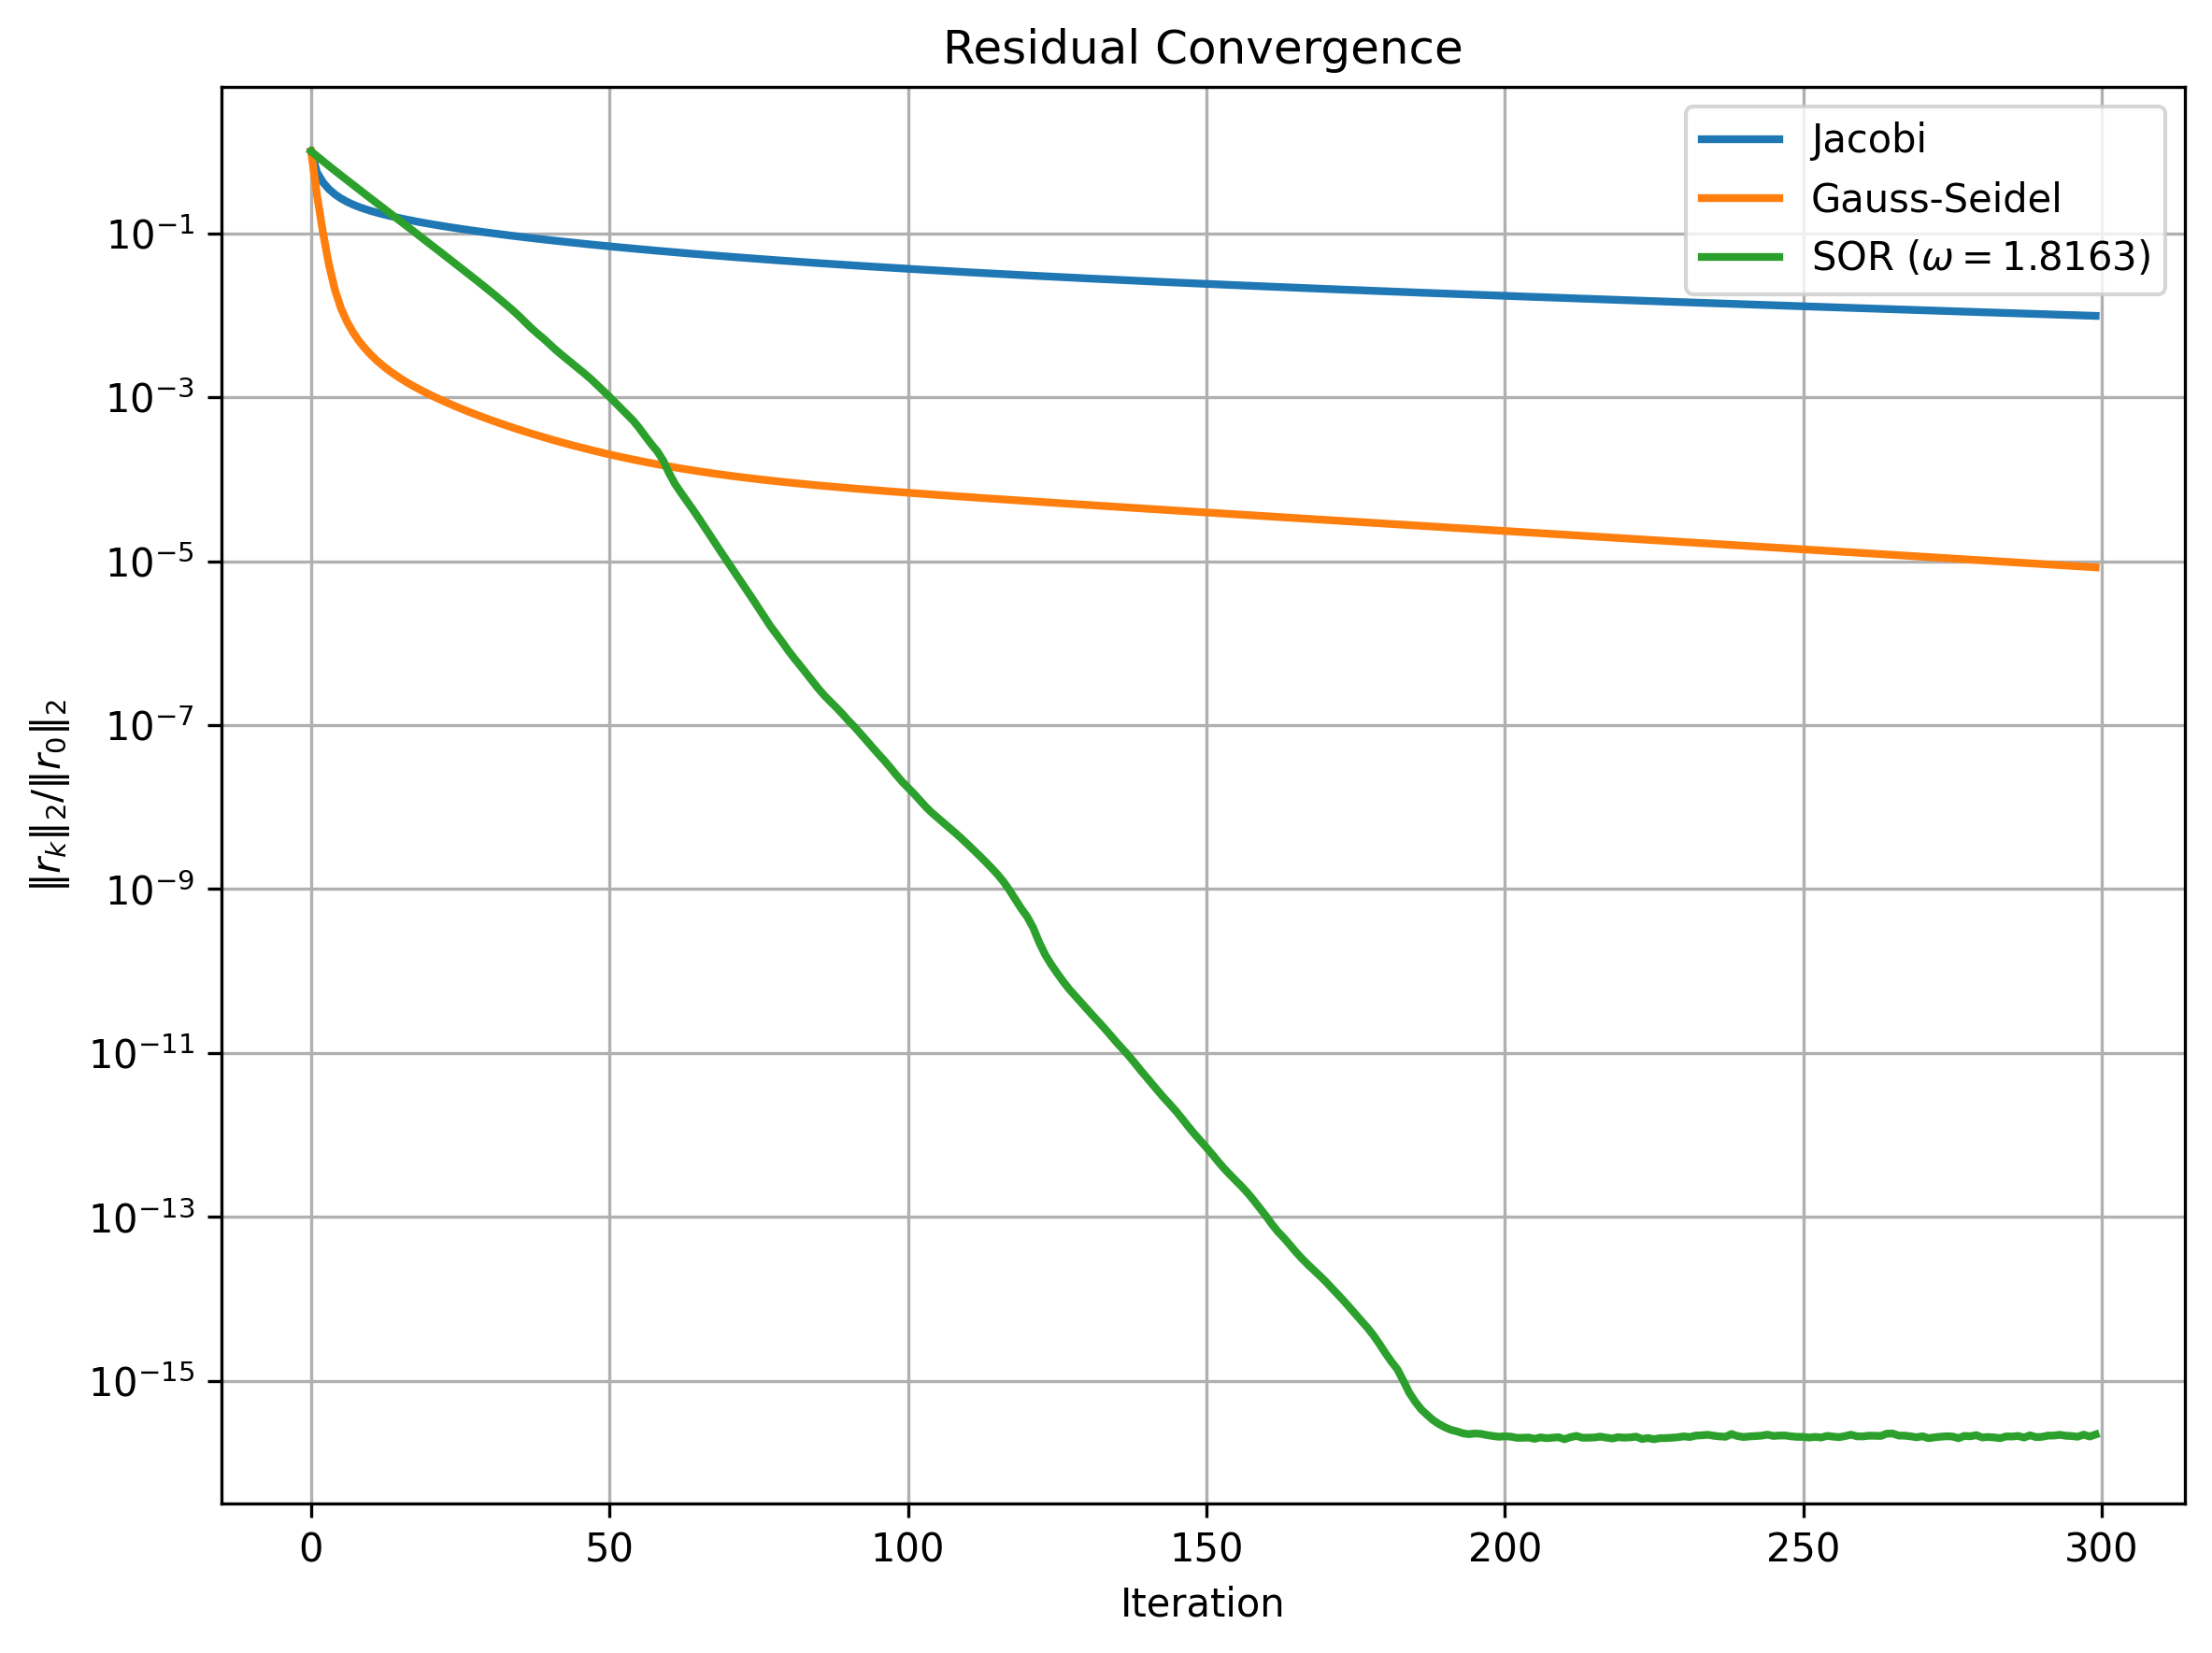
\includegraphics[width=0.75\textwidth]
        {figure1_residual_convergence.png}
        \caption{Relative residual histories of Jacobi, Gauss--Seidel and optimal SOR.}
        \label{fig:residual}
      \end{figure}

      From Figure~\ref{fig:residual}, the Jacobi iteration converges most
      slowly, the Gauss--Seidel iteration is slightly faster, and the optimal
      SOR iteration converges significantly faster than both. This agrees with
      the theoretical ordering

      \[
        \rho_{SOR}
        <
        \rho_{GS}
        <
        \rho_J.
      \]

      To further verify Young's theory, we plot

      \[
        q_k
        =
        \frac{\norm{r_{k+1}}_2}{\norm{r_k}_2},
      \]

      together with the theoretical spectral radii.

      \begin{figure}[htbp]
        \centering
        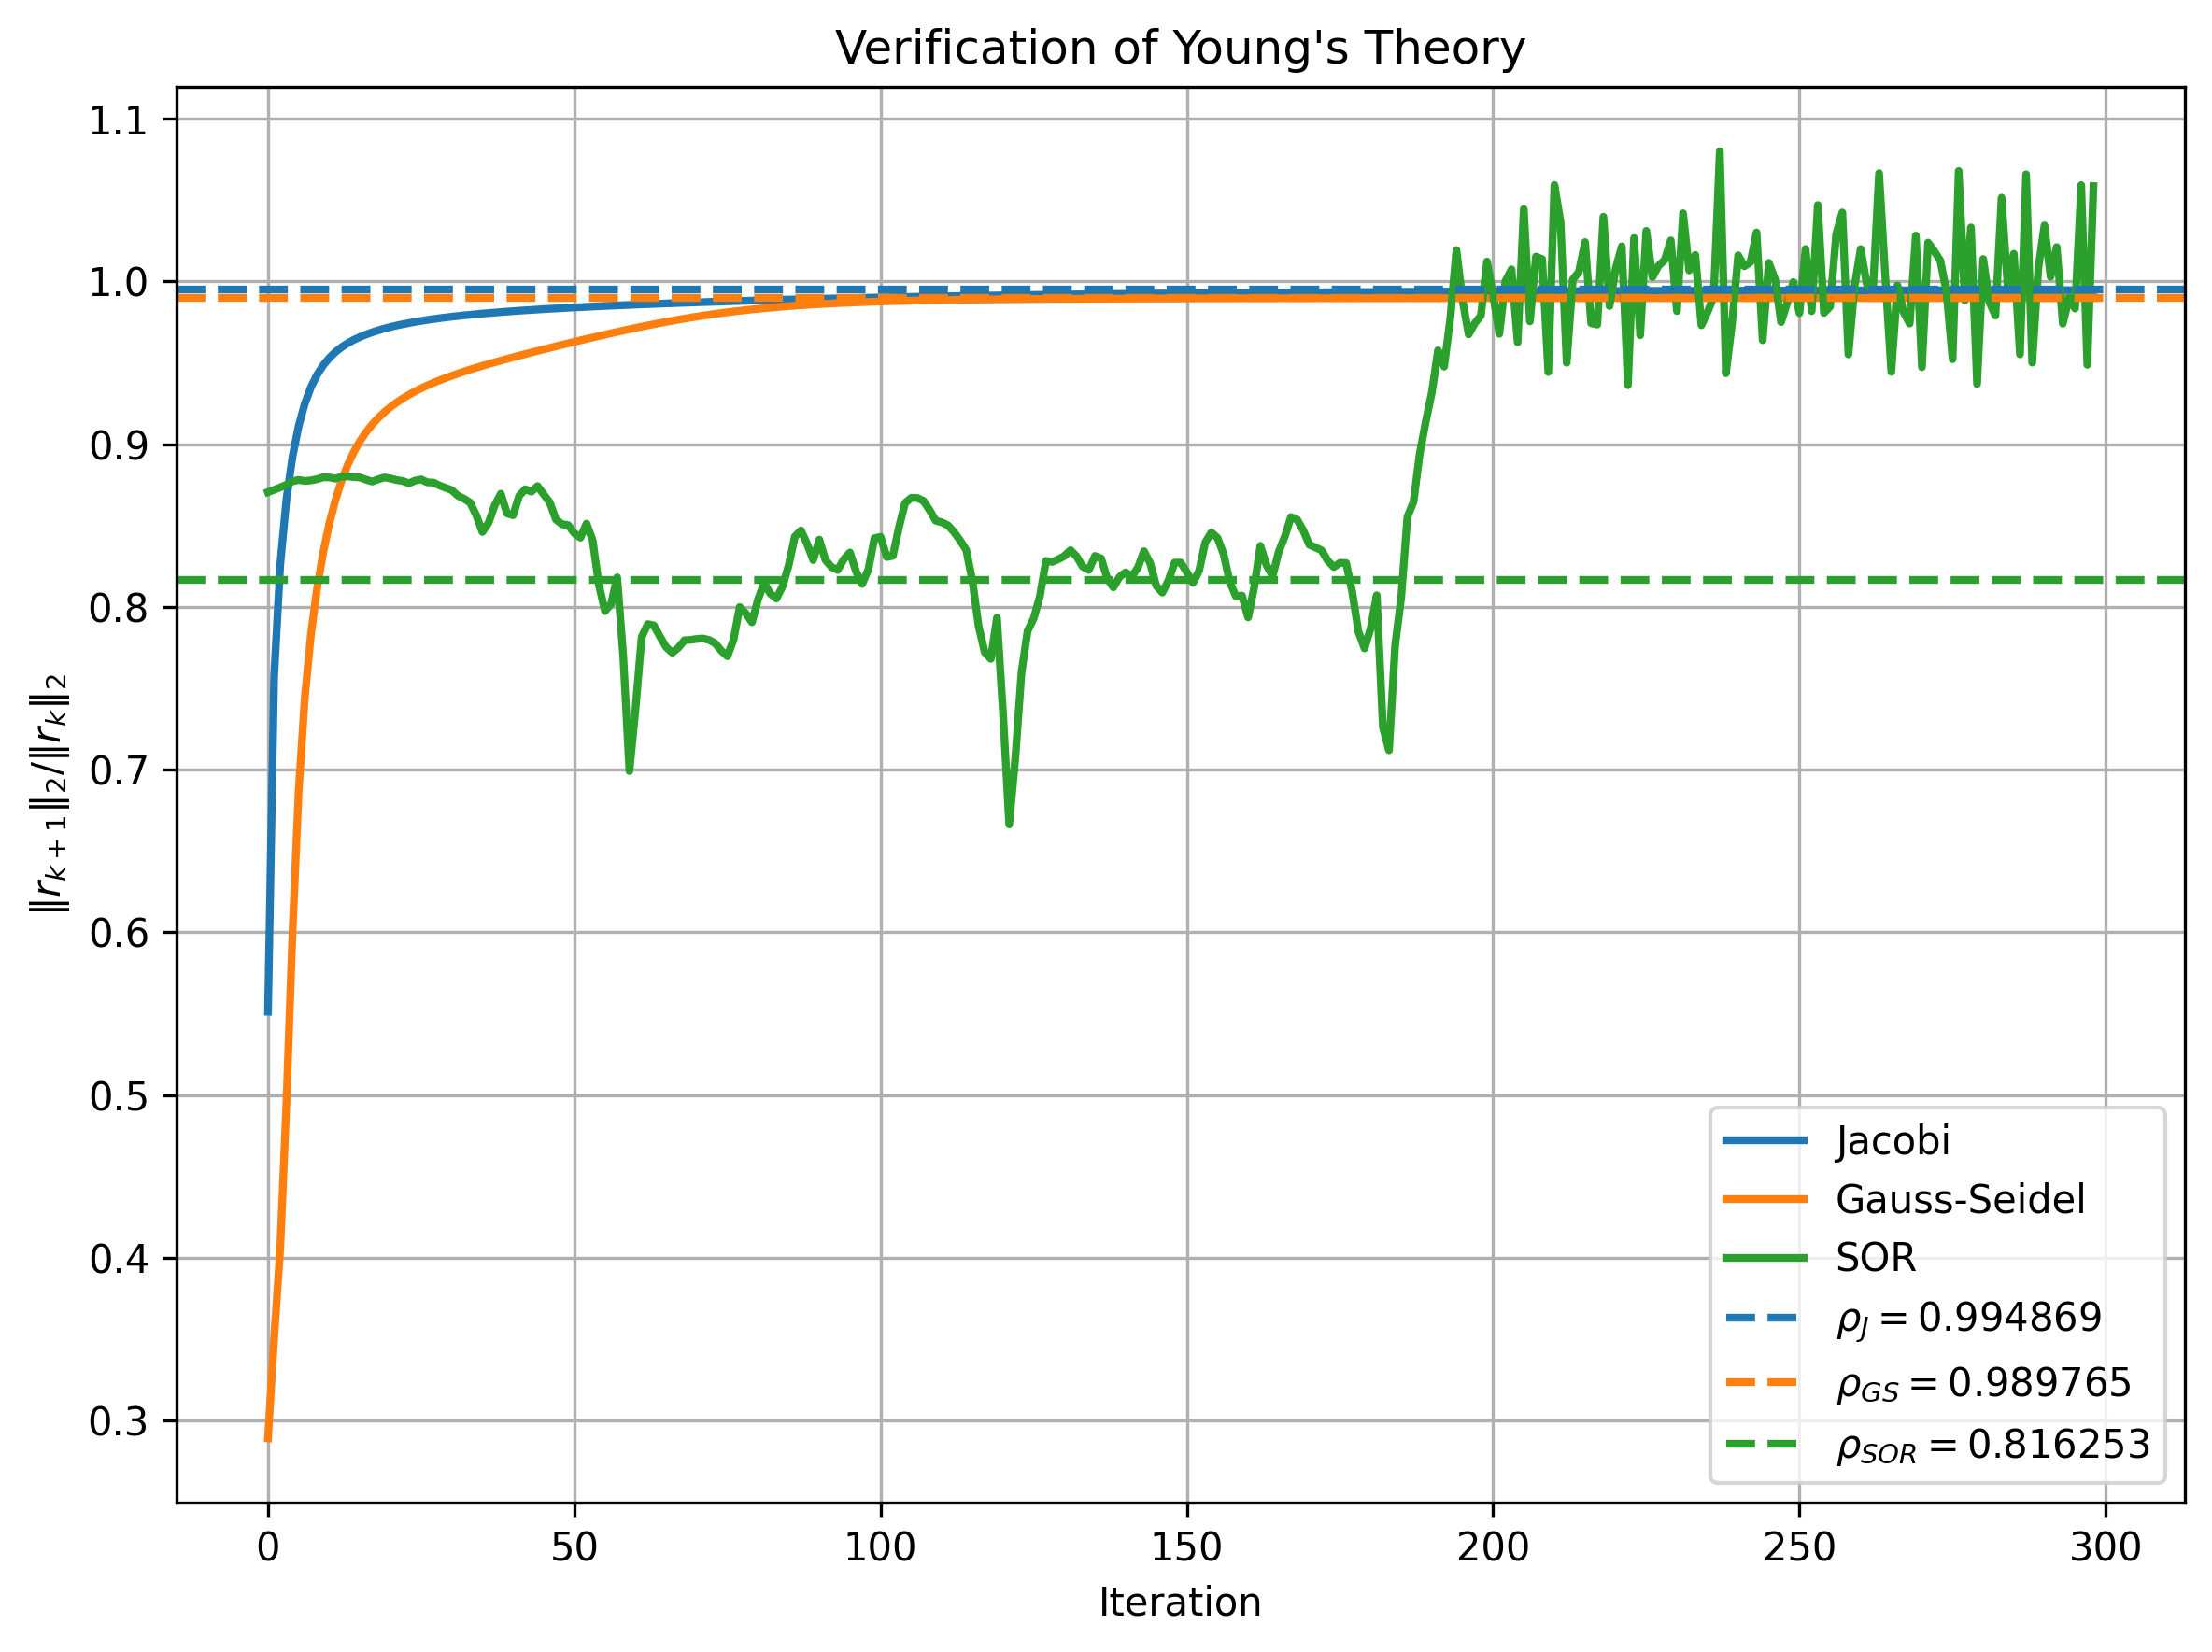
\includegraphics[width=0.75\textwidth]
        {figure2_verify_young.png}
        \caption{Observed convergence factors and theoretical spectral radii.}
        \label{fig:young}
      \end{figure}

      For Jacobi and Gauss--Seidel, the observed asymptotic convergence
      factors are

      \[
        q_J
        \approx
        0.99459726,
        \qquad
        q_{GS}
        \approx
        0.98975788,
      \]

      which are very close to

      \[
        \rho_J
        =
        0.99486932,
        \qquad
        \rho_{GS}
        =
        0.98976497.
      \]

      In particular,

      \[
        \rho_{GS}
        =
        \rho_J^2,
      \]

      which is exactly the relation predicted by Young's theorem for matrices
      having Property~A.

      For the SOR method, the residual decreases rapidly to the level of
      machine precision. Consequently, the quantity

      \[
        \frac{\norm{r_{k+1}}_2}{\norm{r_k}_2}
      \]

      is eventually dominated by round-off errors and no longer provides a
      reliable estimate of the asymptotic convergence factor. Therefore, only
      the initial asymptotic regime should be used for comparison with the
      theoretical value

      \[
        \rho_{SOR}
        =
        0.81625276.
      \]

      Overall, the numerical results agree with Young's theory and confirm the
      predicted convergence behavior of Jacobi, Gauss--Seidel, and optimal
      SOR iterations for the five-point approximation matrix.
  \end{enumerate}

\end{solution}
\begin{problem}\label{pro:7}
  \begin{enumerate}
    \item
      \(
        |A^k| \le |A|^k
        \qquad \text{for all } k=1,2,\ldots
      \)

    \item
      If
      \(
        0 \le A \le B,
      \)
      then
      \[
        0 \le A^k \le B^k
        \qquad \text{for all } k=1,2,\ldots
      \]

    \item
      If
      \(
        A>0,
      \)
      then
      \[
        A^k>0
        \qquad \text{for all } k=1,2,\ldots
      \]

    \item
      If
      \(
        A>0,v\ge 0,
      \)
      and \(v\) is not the zero vector, then
      \(
        Av>0.
      \)

    \item
      If
      \(
        A\ge 0, v\ge 0,
      \)
      and
      \(
        Av\ge \alpha v
      \)
      for some \(\alpha>0\), then
      \[
        A^k v \ge \alpha^k v
        \qquad \text{for all } k=1,2,\ldots
      \]
  \end{enumerate}
\end{problem}
\begin{solution}
  Let \(A=(a_{ij})\).

  \begin{enumerate}
    \item[(a)]
      We prove that
      \[
        |A^k|\le |A|^k,\qquad k=1,2,\ldots .
      \]

      For \(k=1\), the result is obvious. Suppose that
      \[
        |A^k|\le |A|^k.
      \]
      Then
      \[
        |A^{k+1}|
        =|A^kA|
        \le |A^k|\,|A|
        \le |A|^k|A|
        =|A|^{k+1}.
      \]
      Hence, by induction,
      \[
        |A^k|\le |A|^k
      \]
      for all \(k=1,2,\ldots\).
    \item[(b)]
      Assume that
      \[
        0\le A\le B.
      \]
      We prove that
      \[
        0\le A^k\le B^k,\qquad k=1,2,\ldots .
      \]

      Since \(A\ge0\), every entry of \(A^k\) is a sum of products of
      nonnegative numbers. Hence
      \[
        A^k\ge0.
      \]

      Now for each \(i,j\), we write the \((i,j)\)-entry of \(A^k\) as
      \[
        (A^k)_{ij}
        =
        \sum_{i_1,\ldots,i_{k-1}}
        a_{i i_1}a_{i_1 i_2}\cdots a_{i_{k-1}j}.
      \]
      Similarly,
      \[
        (B^k)_{ij}
        =
        \sum_{i_1,\ldots,i_{k-1}}
        b_{i i_1}b_{i_1 i_2}\cdots b_{i_{k-1}j}.
      \]

      Because
      \[
        0\le a_{pq}\le b_{pq}
      \]
      for all \(p,q\), we have
      \[
        a_{i i_1}a_{i_1 i_2}\cdots a_{i_{k-1}j}
        \le
        b_{i i_1}b_{i_1 i_2}\cdots b_{i_{k-1}j}.
      \]
      Therefore,
      \[
        (A^k)_{ij}\le (B^k)_{ij}.
      \]

      Since this holds for every \(i,j\), we obtain
      \[
        0\le A^k\le B^k.
      \]

      Thus
      \[
        0\le A^k\le B^k,\qquad k=1,2,\ldots .
      \]

    \item[(c)]
      Assume
      \[
        A>0.
      \]
      We prove that
      \[
        A^k>0,\qquad k=1,2,\ldots .
      \]

      For \(k=1\), this is the assumption. Suppose \(A^k>0\). Then for every \(i,j\),
      \[
        (A^{k+1})_{ij}
        =(A^kA)_{ij}
        =\sum_{\ell}(A^k)_{i\ell}a_{\ell j}.
      \]
      Since \((A^k)_{i\ell}>0\) and \(a_{\ell j}>0\), every term in the sum is positive. Hence
      \[
        (A^{k+1})_{ij}>0.
      \]
      Thus \(A^{k+1}>0\). By induction,
      \[
        A^k>0
      \]
      for all \(k=1,2,\ldots\).

    \item[(d)]
      Assume
      \[
        A>0,\qquad v\ge0,\qquad v\ne0.
      \]
      We prove that
      \[
        Av>0.
      \]

      Since \(v\ge0\) and \(v\ne0\), there exists an index \(j_0\) such that
      \[
        v_{j_0}>0.
      \]
      For each \(i\),
      \[
        (Av)_i=\sum_j a_{ij}v_j.
      \]
      Because \(A>0\), we have \(a_{ij_0}>0\). Therefore
      \[
        (Av)_i
        =\sum_j a_{ij}v_j
        \ge a_{ij_0}v_{j_0}>0.
      \]
      Hence every component of \(Av\) is positive, so
      \[
        Av>0.
      \]

    \item[(e)]
      Assume that
      \[
        A\ge 0,\qquad v\ge 0,\qquad Av\ge \alpha v,
      \]
      where \(\alpha>0\). We prove that
      \[
        A^k v\ge \alpha^k v,\qquad k=1,2,\ldots .
      \]

      For \(k=1\), the conclusion is exactly the assumption:
      \[
        Av\ge \alpha v.
      \]

      Now suppose that for some \(k\ge1\),
      \[
        A^k v\ge \alpha^k v.
      \]
      Then
      \[
        A^k v-\alpha^k v\ge0.
      \]
      Since \(A\ge0\), multiplying a nonnegative vector by \(A\) still gives a nonnegative vector. Hence
      \[
        A(A^k v-\alpha^k v)\ge0.
      \]
      Therefore
      \[
        A^{k+1}v-\alpha^k Av\ge0,
      \]
      so
      \[
        A^{k+1}v\ge \alpha^k Av.
      \]
      Using the assumption \(Av\ge \alpha v\), we get
      \[
        A^{k+1}v
        \ge \alpha^k Av
        \ge \alpha^k \alpha v
        =\alpha^{k+1}v.
      \]

      Thus, by induction,
      \[
        A^k v\ge \alpha^k v,\qquad k=1,2,\ldots .
      \]
  \end{enumerate}
\end{solution}
\begin{problem}\label{pro:8}
  Show that the iterates $x_k$ generated by the PCG algorithm with
  preconditioner $M$ are the same as those generated with
  preconditioner $cM$ for any $c>0$.
\end{problem}

We provide \(2 \) perspective to solve the problem.
\begin{solution}
  Consider the PCG method applied to the linear system
  \[
    Ax=b,
  \]
  with preconditioner \(M\). Let
  \[
    r_k=b-Ax_k,\qquad Mz_k=r_k.
  \]
  Equivalently,
  \[
    z_k=M^{-1}r_k.
  \]

  If the preconditioner is changed from \(M\) to \(cM\), where \(c>0\), then
  the corresponding preconditioned residual \(\widetilde z_k\) satisfies
  \[
    (cM)\widetilde z_k=r_k.
  \]
  Hence
  \[
    \widetilde z_k=(cM)^{-1}r_k
    =\frac{1}{c}M^{-1}r_k
    =\frac{1}{c}z_k.
  \]

  In the PCG algorithm, the step size is
  \[
    \alpha_k=\frac{r_k^Tz_k}{p_k^TAp_k}.
  \]
  For the preconditioner \(cM\), the numerator becomes
  \[
    r_k^T\widetilde z_k
    =
    r_k^T\left(\frac{1}{c}z_k\right)
    =
    \frac{1}{c}r_k^Tz_k.
  \]

  We now show that the search directions are scaled by the same factor.
  For \(k=0\),
  \[
    \widetilde p_0=\widetilde z_0=\frac{1}{c}z_0=\frac{1}{c}p_0.
  \]
  Assume that
  \[
    \widetilde p_k=\frac{1}{c}p_k.
  \]
  Then
  \[
    \widetilde p_k^TA\widetilde p_k
    =
    \left(\frac{1}{c}p_k\right)^T
    A
    \left(\frac{1}{c}p_k\right)
    =
    \frac{1}{c^2}p_k^TAp_k.
  \]
  Therefore the step size for the preconditioner \(cM\) is
  \[
    \widetilde\alpha_k
    =
    \frac{r_k^T\widetilde z_k}
    {\widetilde p_k^TA\widetilde p_k}
    =
    \frac{(1/c)r_k^Tz_k}{(1/c^2)p_k^TAp_k}
    =
    c\alpha_k.
  \]

  Thus
  \[
    \widetilde\alpha_k\widetilde p_k
    =
    (c\alpha_k)\left(\frac{1}{c}p_k\right)
    =
    \alpha_kp_k.
  \]
  Hence
  \[
    \widetilde x_{k+1}
    =
    \widetilde x_k+\widetilde\alpha_k\widetilde p_k
    =
    x_k+\alpha_kp_k
    =
    x_{k+1}.
  \]
  So the iterates \(x_k\) are unchanged.

  It remains to check that the next search direction has the same scaling.
  The residual update is
  \[
    r_{k+1}=r_k-\alpha_kAp_k.
  \]
  Since
  \[
    \widetilde\alpha_k\widetilde p_k=\alpha_kp_k,
  \]
  we also have
  \[
    \widetilde r_{k+1}=r_{k+1}.
  \]
  Therefore
  \[
    \widetilde z_{k+1}
    =
    (cM)^{-1}r_{k+1}
    =
    \frac{1}{c}z_{k+1}.
  \]
  The coefficient \(\beta_k\) is
  \[
    \beta_k=\frac{r_{k+1}^Tz_{k+1}}{r_k^Tz_k}.
  \]
  For the scaled preconditioner,
  \[
    \widetilde\beta_k
    =
    \frac{r_{k+1}^T\widetilde z_{k+1}}
    {r_k^T\widetilde z_k}
    =
    \frac{(1/c)r_{k+1}^Tz_{k+1}}
    {(1/c)r_k^Tz_k}
    =
    \beta_k.
  \]
  Thus
  \[
    \widetilde p_{k+1}
    =
    \widetilde z_{k+1}
    +
    \widetilde\beta_k\widetilde p_k
    =
    \frac{1}{c}z_{k+1}
    +
    \beta_k\frac{1}{c}p_k
    =
    \frac{1}{c}p_{k+1}.
  \]
  By induction, the search directions are scaled by \(1/c\), while the step
  sizes are scaled by \(c\). Their product is unchanged, so the iterates
  \(x_k\) generated by PCG with preconditioner \(M\) and \(cM\) are the same.
\end{solution}
\begin{solution}
  Let
  \[
    r_0=b-Ax_0.
  \]

  For the preconditioner \(M\), the preconditioned matrix is

  \[
    B=M^{-1}A.
  \]

  For the scaled preconditioner \(cM\), \(c>0\), the corresponding
  preconditioned matrix is

  \[
    \widetilde B=(cM)^{-1}A
    =\frac1c\,M^{-1}A
    =\frac1c B.
  \]

  The \(k\)-th Krylov subspace generated by \(B\) is

  \[
    \mathcal K_k(B,r_0)
    =
    \operatorname{span}
    \{r_0,Br_0,\ldots,B^{k-1}r_0\}.
  \]

  Similarly,

  \[
    \mathcal K_k(\widetilde B,r_0)
    =
    \operatorname{span}
    \{r_0,\widetilde Br_0,\ldots,\widetilde B^{k-1}r_0\}.
  \]

  Since

  \[
    \widetilde B^j
    =
    \left(\frac1c B\right)^j
    =
    \frac1{c^j}B^j,
  \]

  we obtain

  \[
    \mathcal K_k(\widetilde B,r_0)
    =
    \operatorname{span}
    \left\{
      r_0,
      \frac1cBr_0,
      \ldots,
      \frac1{c^{k-1}}B^{k-1}r_0
    \right\}.
  \]

  Multiplying basis vectors by nonzero scalars does not change the span,
  hence

  \[
    \mathcal K_k(\widetilde B,r_0)
    =
    \mathcal K_k(B,r_0).
  \]

  Therefore both PCG methods generate exactly the same Krylov subspaces.

  A fundamental characterization of PCG states that \(x_k\) is the unique
  vector in

  \[
    x_0+\mathcal K_k(B,r_0)
  \]

  whose error is \(A\)-orthogonal to the Krylov subspace; equivalently,

  \[
    x_k
    =
    \operatorname*{arg\,min}_{x\in x_0+\mathcal K_k(B,r_0)}
    \norm{x-x_*}_A.
  \]

  Since the two methods have the same initial guess \(x_0\), the same
  matrix \(A\), and the same Krylov subspace at every iteration,
  the minimization problem defining \(x_k\) is identical in both cases.

  Consequently,

  \[
    \widetilde x_k=x_k,
    \qquad k=0,1,2,\ldots.
  \]

  Hence the iterates generated by PCG with preconditioners \(M\) and
  \(cM\) are identical.
\end{solution}
\begin{problem}\label{pro:9}
  The multigroup transport equation can be written in the form
  \[
    \Omega \cdot \nabla \psi_g
    +\sigma_g \psi_g
    -\sum_{g'=1}^{G}
    \int_{S^2}
    \sigma_{g,g'}(r,\Omega\cdot\Omega')
    \,\psi_{g'}(r,\Omega')
    \,d\Omega'
    =
    f_g,
    \qquad
    g=1,\ldots,G,
  \]
  where $\psi_g(r,\Omega)$ is the unknown flux associated with energy group $g$ and
  $\sigma_g(r,\Omega)$, $\sigma_{g,g'}(r,\Omega\cdot\Omega')$, and
  $f_g(r,\Omega)$ are known cross-section and source terms.
  (Appropriate boundary conditions are also given.)

  A standard method for solving this set of equations is to move the terms
  of the sum corresponding to different energy groups to the right-hand side
  and solve the resulting set of equations for
  $\psi_1,\ldots,\psi_G$ in increasing order of index, using the most
  recently updated quantities on the right-hand side; that is,
  \[
    (\Omega\cdot\nabla+\sigma_g)\psi_g^{(k)}
    -
    \int_{S^2}
    \sigma_{g,g}\,\psi_g^{(k)}
    \,d\Omega'
    =
    f_g
    +
    \sum_{g'<g}
    \int_{S^2}
    \sigma_{g,g'}\,\psi_{g'}^{(k)}
    \,d\Omega'
    +
    \sum_{g'>g}
    \int_{S^2}
    \sigma_{g,g'}\,\psi_{g'}^{(k-1)}
    \,d\Omega'.
  \]

  Identify this procedure with one of the preconditioned iterative methods
  described in the lectures. How might it be accelerated?
\end{problem}
\begin{solution}
  Let
  \[
    \psi=(\psi_1,\psi_2,\ldots,\psi_G)^T
  \]
  be the vector of all unknown group fluxes.  This means that instead of
  treating the $G$ equations separately, we regard all fluxes as one large
  unknown vector.

  Define the diagonal block operator
  \[
    A_{gg}\psi_g
    =
    (\Omega\cdot\nabla+\sigma_g)\psi_g
    -
    \int_{S^2}\sigma_{g,g}\psi_g\,d\Omega'.
  \]
  This is the part of the $g$-th equation that involves only the unknown
  $\psi_g$ itself, so it represents the within-group transport operator.

  For $g'\neq g$, define the off-diagonal coupling operators
  \[
    A_{gg'}\psi_{g'}
    =
    -\int_{S^2}\sigma_{g,g'}\psi_{g'}\,d\Omega'.
  \]
  These terms describe the coupling from energy group $g'$ to energy group
  $g$.

  With these definitions, the multigroup transport equations can be written
  as one block linear system
  \[
    A\psi=f.
  \]

  Now split the block operator $A$ as
  \[
    A=D-L-U,
  \]
  where $D$ contains the diagonal blocks $A_{gg}$, $L$ contains the
  strictly lower-triangular block part, and $U$ contains the strictly
  upper-triangular block part.

  In the given procedure, when solving for $\psi_g^{(k)}$, the quantities
  $\psi_{g'}^{(k)}$ with $g'<g$ have already been updated in the current
  sweep, while the quantities $\psi_{g'}^{(k-1)}$ with $g'>g$ have not yet
  been updated and therefore are taken from the previous iteration.

  Therefore the iteration can be written in block form as
  \[
    (D-L)\psi^{(k)}=f+U\psi^{(k-1)}.
  \]
  Equivalently,
  \[
    \psi^{(k)}
    =
    (D-L)^{-1}f
    +
    (D-L)^{-1}U\psi^{(k-1)}.
  \]

  This is exactly the block Gauss--Seidel iteration, because the unknowns
  are updated successively in the order $g=1,2,\ldots,G$, and the newest
  available values are immediately used.

  From the viewpoint of preconditioned iterative methods, set
  \[
    M=D-L.
  \]
  Then the iteration can also be written as
  \[
    \psi^{(k)}
    =
    \psi^{(k-1)}
    +
    M^{-1}\bigl(f-A\psi^{(k-1)}\bigr).
  \]
  Indeed, since
  \[
    A=D-L-U=M-U,
  \]
  we have
  \[
    f-A\psi^{(k-1)}
    =
    f-(M-U)\psi^{(k-1)}
    =
    f-M\psi^{(k-1)}+U\psi^{(k-1)}.
  \]
  Hence
  \[
    \psi^{(k-1)}
    +
    M^{-1}\bigl(f-A\psi^{(k-1)}\bigr)
    =
    M^{-1}f+M^{-1}U\psi^{(k-1)},
  \]
  which is the same iteration as above.

  Thus the procedure is a preconditioned Richardson iteration with the
  block Gauss--Seidel preconditioner
  \[
    M=D-L.
  \]
  Equivalently, it is the block Gauss--Seidel method applied to the
  multigroup transport system.

  A natural way to accelerate the procedure is to use the same operator
  \[
    M=D-L
  \]
  as a preconditioner in a Krylov subspace method, such as GMRES, GCR, or
  BiCGSTAB.  For example, one may solve the left-preconditioned system
  \[
    M^{-1}A\psi=M^{-1}f.
  \]
  Applying $M^{-1}$ corresponds to one forward sweep through the energy
  groups, so the preconditioner is natural and relatively inexpensive.
  The Krylov method then accelerates the convergence compared with the
  stationary block Gauss--Seidel iteration.

  Therefore,
  \[
    \boxed{
      \text{the procedure is block Gauss--Seidel, or equivalently
      preconditioned Richardson with } M=D-L,
    }
  \]
  and it can be accelerated by Krylov methods such as GMRES using this
  block Gauss--Seidel sweep as a preconditioner.
\end{solution}
\end{document}
